% !TEX root = /home/Documents/thesis/draft/thesis.tex
\documentclass[12pt,twoside]{reedthesis}

\usepackage{graphicx,latexsym}
\usepackage{amssymb,amsthm,amsmath}
\usepackage{longtable,booktabs,setspace}
\usepackage[hyphens]{url}
\usepackage{rotating}
\usepackage{listings}
\usepackage{float}
\usepackage{fancyvrb}
\usepackage{hyperref}
\usepackage{xcolor}
\usepackage{tikz}
\usepackage[backend=biber, style=numeric, sorting=ynt]{biblatex}
\addbibresource{thesis.bib}

\newcommand{\revise}[1]{{\color{red}#1}}
\newcommand{\vstep}{\vspace{5mm}}

\lstset{	% for source code formatting
basicstyle=\small\ttfamily,
columns=flexible,
breaklines=true
}

\title{A Continued Inquiry into Granularity-Change Cache Simulation}
\author{Alan R. Jessup}
% The month and year that you submit your FINAL draft TO THE LIBRARY (May or December)
\date{May 2024}
\division{Mathematics and Natural Sciences}
\advisor{Charles McGuffey}
\department{Computer Science}

\setlength{\parskip}{0pt}
\begin{document}

\maketitle
\frontmatter % this stuff will be roman-numbered
\pagestyle{empty}

\tableofcontents

% If your abstract is longer than a page, there may be a formatting issue.
\chapter*{Abstract}

The 2021 paper ``Spatial Locality and Granularity Change in Caching'' presented the Granularity-Change Caching Problem, the study of a cache architecture in which the shift in data granularity between the cache and main memory is utilized to load additional spatially local data without additional cost. The paper provided theoretical analysis of the granularity-change caching problem and described the replacement policy Item-Block Layered Partitioning (IBLP) to implement a simple granularity-change cache \cite{beckmann}.

To study the performance of granularity-change caching in practice, the 2022 Reed thesis ``Simulating the Granularity-Change Caching Problem'' used the open-source system simulator Gem5 to provide the first simulated implementation and analysis of an IBLP cache, and suggested areas for continued research toward a more realistic and versatile simulation \cite{curtis}.

My research continues to build on the prior work in granularity-change cache simulation by introducing a new strategy to implement granularity-change caching in Gem5 and by evaluating the limitations of the three available approaches to this strategy. I find that this method of implementing a granularity-change cache in Gem5 is not possible without expanding the features of the Gem5 simulator as a whole, and provide a cursory look at what such modifications would involve.

\mainmatter
\pagestyle{fancyplain}

\chapter{Introduction}

\section{Significance}

Computer caching is crucial to the efficient performance of data retrieval in modern computer memory systems. As processor technology improves and computers are able to generate requests for stored data significantly faster than those requests can be served, advancements in caching provide the valuable opportunity to improve memory access speed and therefore overall efficiency.

The 2021 paper ``Spatial Locality and Granularity Change in Caching'' introduced a cache configuration called the Granularity-Change Cache, which takes advantage of the granularity at which data is accessed in order to load additional data into the cache at little to no additional cost.

Developing a simulation of a Granularity-Change cache would benefit research in computer caching by providing a tool to gain greater insight into the impacts and uses of spatial locality. Analysis using such a simulation could help determine the viability of granularity-change caches for implementation in real computer systems.

To this effect, the 2022 thesis ``Simulating the Granularity-Change Caching Problem'' by Maxx Curtis explored the possibility of simulating a granularity-change cache using the powerful systems simulation platform Gem5. This work provided a foundation for studying granularity-change cache simulation by presenting implementation and testing of a potential granularity-change cache implementation in Gem5, and indicated that granularity-change cache simulation is an area where further research would be beneficial.

\section{Approach}

	% curtis findings
	In describing suggestions for future work, Curtis states: \begin{quote}
		At this stage of development, I recommend against using my implementation for further research into IBLP. ... If one only wanted to examine the viability of IBLP itself, then it would be fairly easy to use typical Cache objects to do so... by creating a system with two caches, one for each layer, that differ in granularity and experience little to no intermediate latency \cite{curtis}.
	\end{quote}

	Furthermore, the repository linked as containing the code used in the Curtis thesis does not contain any of said code, so expanding on the block cache implementation is not an option.

	Curtis also suggests working towards an implementation of a granularity-change cache model that is compatible with more realistic processors than Gem5's simple CPU models. Since Gem5 has a wide variety of available CPU models, this is a matter of compatibility with the full array of cache features in Gem5, including response queues and cache coherence.

	% approach
	With the results and suggestions of the Curtis thesis in mind, my approach to further research on the granularity-change caching problem was to build and test a modular implementation of IBLP using the existing Gem5 cache objects. Since the existing Gem5 caches are compatible with the full range of Gem5's features, an implementation using these caches as its foundation would be able to maintain these compatibilities, thereby eliminating the need for laborious re-implementation of Gem5's cache features from the ground up.

\section{Results}

Over multiple different attempted methods of implementing IBLP in Gem5, I uncovered evidence against the viability of each method of implementation. My attempt to implement a nestled cache structure using Gem5's modular classic cache objects revealed the dependence of cache line size on a system-level variable, and thus the impossibility of independently changing the cache line size within one of Gem5's typical caches. My look at a simple cache implementation in Gem5's Ruby memory subsystem revealed similar findings due to the similar dependence on a system object. Finally, my preliminary analysis of Gem5's source code for the classic cache objects provided mixed results that suggest the uncertain possibility and likely difficulty of modifying the Gem5 source code to support granularity change between caches.

Overall, my research has provided strong evidence against the use of Gem5 to simulating the granularity-change caching problem. Between the findings of the Curtis thesis on the impracticality of a ground-up implementation of new CG-cache objects, and my findings on the complications to using existing Gem5 objects to imitate a granularity change, this exhausts the most direct approaches to implementing granularity-change caching in Gem5.


\chapter{Background}

\section{A crash course in computer caching}

Computer memory is the fundamental component of digital systems that serves as a dynamic repository where data and instructions can be temporarily stored for quick access and retrieval during active processes. The much lower latency of memory requests compared to retrieval of data from a hard drive or SSD makes memory crucial to the efficient performance of modern computers.

	\subsection*{The memory hierarchy}

	A computer's various types of storage make up the memory hierarchy; layers of storage are arranged in tiers of the hierarchy based on size and access speed, with faster but smaller and more expensive layers of memory at the top of the hierarchy, and slower, larger storage at the bottom. When the processor requests data from memory, each layer of the hierarchy is checked in descending order until the data is located, so that fewer checks are made to the lower, slower memory than to the higher, faster layers.

	\begin{figure}[h]
    	\centering
    	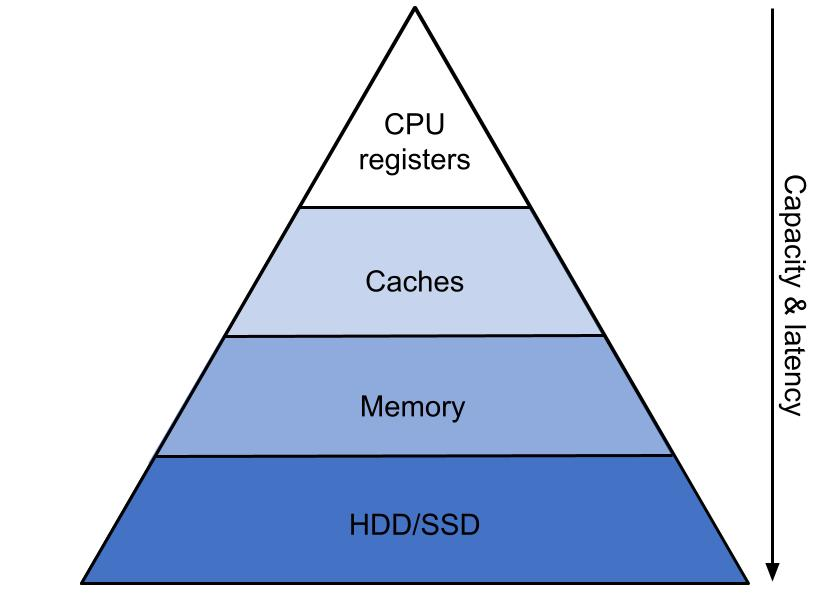
\includegraphics[width=3.5in]{figures/mem_hierarchy.jpg}
    	\caption{A diagram of the memory hierarchy.}
	\end{figure}

	\subsection*{Basics of caching}
	
	The purpose of caching is to reduce the number of accesses made to the main memory by storing select pieces of data that are most likely to be requested in the near future. When a piece of requested data is present in a cache, that is called a cache hit; when it is absent, it's a cache miss. Since caches are small and fast, intended to be accessed frequently at minimal cost, an important factor of cache design is how to best utilize the limited space they offer to optimize the hit rate, i.e. the percent of total requests for which the requested data is present in the cache.
	
	The algorithms used to optimize hit rate by determining which data to admit to and evict from a cache are called replacement policies. Replacement policies are designed using properties of data called spatial and temporal locality.

	\subsection*{Data locality}
	
	Temporal locality applies to data that has been used recently, and therefore is typically more likely to be needed again than some arbitrary other piece of data. Temporal locality is central to many replacement policies, such as a the Least Recently Used (LRU) policy which, upon loading a new piece of data from main memory, chooses data in the cache to evict by which data was least recently requested by the processor.
	
	Spatial locality applies to data that is located physically near other useful data in memory. Caches operate on sections of data called lines (or blocks), where a cache's line size determines the granularity of the cache. A cache will load an entire line (usually 32, 64, or 128 bytes) when any piece of data stored within that line in requested. A cache's utilization of spatial locality corresponds to the line size of the cache; a larger line size loads more data which is located near the specific requested item, and thus populates the cache with this peripheral data that is spatially local.

%	\subsection*{Further concepts in caching}

%	A variety of other design choices impact cache performance, particularly in more complex multiprocessor systems. Cache coherence refers to protocols used to keep multiple caches that store the same data consistent with each other. Inclusive caches are caches which contain data also present in lower levels of memory, and which also require cache coherence with lower layers, whereas exclusive caches contain no duplicate data and thus require a method of tracking to prevent duplication.


\section{The granularity-change caching problem}

According the 2021 paper ``Spatial Locality and Granularity Change in Caching'' by Beckmann et. al., spatial locality is much less well-studied than temporal locality  \cite{beckmann}. Beckmann et. al. aims to improve understanding of spatial locality through the introduction of the Granularity-Change Caching Problem.

The Granularity-Change Caching Problem describes a cache configuration with two layers of granularity at which data can be accessed, referred to as ``item granularity'' and ``block\footnote{The use of the term ``block'' in the context of the granularity-change caching problem is separate from the common use of ``block'' as a synonym for ``line'', as mentioned prior. In this thesis, ``block'' will always refer to the granularity-change caching meaning, with the exception of a few cases of variable names quoted from preexisting code referring to the common meaning.} granularity'', with an item begin equivalent to a cache line and a block being equivalent to a group of multiple cache lines that are treated as as a single larger-granularity line, ``such that a cache can choose any subset of a block to load for the same cost as loading any individual item in the block'' \cite{beckmann}.

The idea behind the granularity-change cache is to take advantage of an existing boundary between the granularity of a cache and main memory to load additional spatially local data that would otherwise be ignored. When an item is requested from memory, the entire page must be loaded, and since cache line size is typically smaller than memory page\footnote{A memory ``page'' is a section of memory, similar to a cache line but specific to lower-level main memory.} size, a portion of that page is ignored---wasting the opportunity to load additional data at little to no additional cost. Whereas using the full memory page by making the cache line size equal to the memory page size would cause spatially local data to dominate the cache, the layered granularity-change cache uses the item layer to maintain greater use of temporal locality while still benefiting from the no-additional-cost spatially local data in the block layer.

In regard to loading a subset of a block, the theoretical analysis in Beckmann et. al. finds that ``to achieve the best competitive ratio, one should load either an entire block or a single item, and nothing in between'' \cite{beckmann}. A competitive ratio is a measurement used in theoretical analysis of cache replacement policies that compares a cache's actual eviction choices in practice (called the ``online algorithm'') with the optimal choices given full knowledge of future requests (called the ``offline algorithm''). The higher the competitive ratio of a cache, the closer its performance is to optimal. For the sake of focusing on the best model for improving cache performance, in this thesis I will be focusing specifically on the subproblem that only involves loading entire blocks and individual items.

Beckmann et. al. describes a simple, deterministic replacement policy for this subproblem called Item-Block Layer Partitioning (IBLP).

	\subsection*{Item-Block Layered Partitioning}

	IBLP divides a cache into two virtual segments, one of item granularity and the other of block granularity, with minimal latency between them. Beckmann et. al. describes the behavior of IBLP as: \begin{quote}
		The first layer, which serves each access to the cache, loads only the items that are accessed and evicts using the Least-Recently Used (LRU) replacement policy. The second layer, which only serves accesses that miss in the first layer, also uses the LRU policy for evictions, but loads and evicts at the granularity of entire blocks at a time \cite{beckmann}.
	\end{quote}

	\begin{figure}[h]
		\centering
		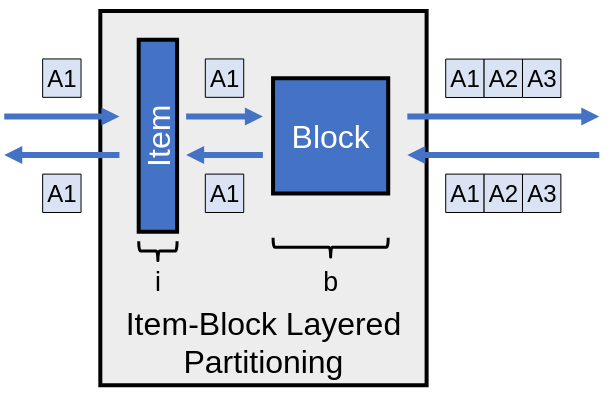
\includegraphics[width=2.5in]{figures/IBLP.png}
		\caption{A diagram of a cache running IBLP \cite{beckmann}.}
	\end{figure}

	This policy provides benefits of both spatial and temporal locality while reducing the tradeoff between the two. By using a separate LRU orderings for each layer, IBLP prevents temporally local data in the item layer from evicting spatially local block layer data.
	
	The block layer is neither inclusive nor exclusive of the item layer, meaning duplicate data may appear in both layers, but data in the item layer is not guaranteed to be present in the block layer. This simplifies the cache's design by preventing need for exclusivity tracking, and maintains the usefulness of the item layer by keeping its contents independent of the block layer \cite{beckmann}. Duplicate data crowding the cache is not expected to have a major performance impact in general cases, since it would only occur if a significant amount of spatially local data was also temporally local, which would overall benefit the hit rate and thus counteract the negative impact caused by loss of cache space.
	
	There is no requirement for the relative sizes $i$ and $b$ of the item and block caches in IBLP. Furthermore, Beckmann et. al. determines the optimal layer sizes in IBLP to be unknown, since they depend on the relative spatial and temporal locality of a particular trace, and recommends further analysis \cite{beckmann}.

\section{Prior work with granularity-change caching}

In 2022, the Reed College thesis titled ``Simulating the Granularity-Change Caching Problem'', by Maxx Curtis, follows-up the theoretical work of Beckmann et. al. on the granularity-change caching problem by providing a foray into practical simulation of the proposed cache model. Curtis provides a survey of two systems simulators, Zsim and Gem5, and a presents a custom implementation of a block Cache in Gem5 \cite{curtis}.

	\subsection*{About the simulators}

	Zsim is a ``fast and accurate microarchitectural simulation'' presented in 2013 \cite{zsim}. Although it showed promise as a tool for simulating granularity-change caching, Curtis finds that a heavy reliance on outsize libraries and lack of continuous support made it difficult and time-consuming to configure.

	Gem5 is an open-source computer systems simulation project with an active development community and emphasis on wide selection of modular system components such as CPU models. It contains two different detailed memory simulation subsystems. The Curtis thesis selects the classic memory subsystem of Gem5 to implement a ``granularity-aware'' block cache for use in IBLP simulation \cite{curtis}.

	\subsection*{Implementation}

	The block cache implemented by Curtis is built from the ground up as a new object, and thus is limited in what features of a Gem5 system it can be configured with. It operates on the level of handling packet streams between the CPU/caches, and facilitates the switch between item and block granularity at this level.

	\subsection*{Limitations}

	The ``Shortcomings'' section of Curtis explains that due to the time-consuming nature of this low-level implementation, the block cache is only usable in simple systems with a single cache level and ``Simple Timing CPU'', a ``unrealistic but very fast CPU model'' \cite{curtis}. Therefore, one suggested area for further research is in creating an implementation of a granularity-change cache that allows for use in more realistic system configurations, such as with Gem5's other more realistic processor models.

	\subsection*{Tests}

	Curtis tests three cache configurations against each other. The control group consists of a simple one-level cache of item granularity and a simple one-level cache using the custom block cache, and the experimental group is an IBLP cache constructed using a standard cache of item granularity in conjunction with a block cache.
	
	\vfill
	\begin{figure}[h]
		\centering
		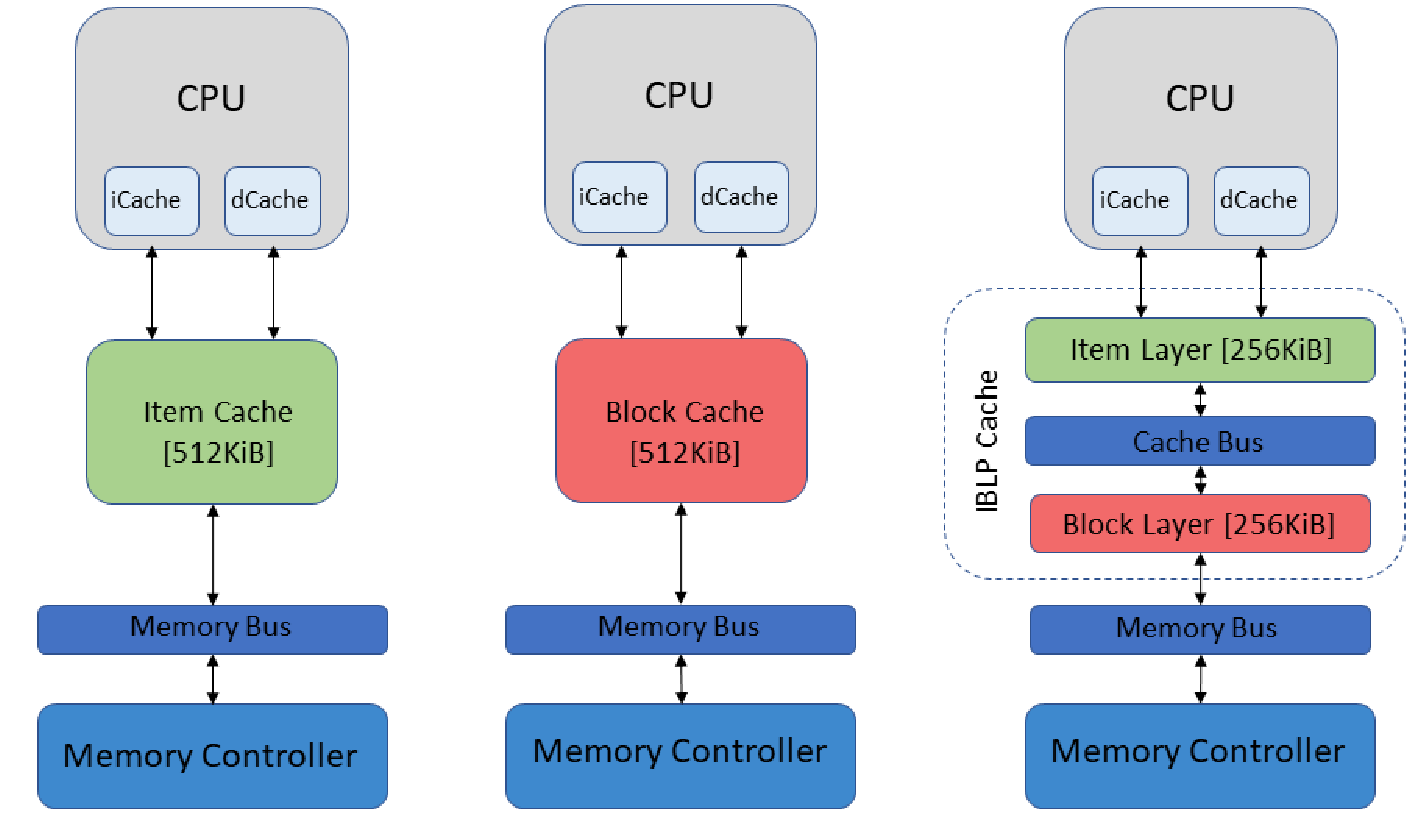
\includegraphics[width=5in]{figures/curtis_caches.png}
		\caption{The three cache configurations tested by Curtis \cite{curtis}.}
	\end{figure}
	\vfill

	Three benchmarks are used: iterative merge sort (high in spatial locality), randomized subset-sum (high in temporal locality), and recursive merge sort (a combination of both forms of locality).
	
	All testing uses an x86 system with Gem5's ``Simple Timing CPU''. Each memory system simulates a 64B line size and 4kiB memory page size, 8GiB of DDR3 for main memory, and a cache size of 512KiB. In IBLP caches, the 512KiB area is divided evenly between the item and block layers \cite{curtis}.

	Each test script is given as input a file with 1 million randomly generated 8-byte values, and gives as output a randomly selected subset of the sorted result to prevent the writing of a large sequential output from skewing the data toward spatial locality \cite{curtis}.

	\subsection*{Results}

	Both merge sort scripts result in a a hit rate near $100\%$ for all three cache types, and randomized subset-sum results in a hit rate near $99.5\%$ for the item and block caches and near $95.5\%$ for the IBLP cache \cite{curtis}. Since outcomes in the control groups do not align with the expectations of poor performance of the item cache for high spatial locality and poor performance of the block cache for high temporal locality, the results of these tests are inconclusive.

	Looking specifically at the hit rates of the individual layers of the IBLP cache, the three test scripts do not support the expectation of a positive corelation between high spatial locality and high relative utilization of the block layer.

	Curtis suggests that these inconclusive results are due in part to the coarse granularity of the block layer in the IBLP cache, and insufficient memory workload of the test scripts compared to the caches' sizes. These factors are thus important to keep in mind when designing future tests to measure performance of granularity-change caches.

	\newpage
	\null
	\vfill

	\begin{figure}[H]
		\centering
		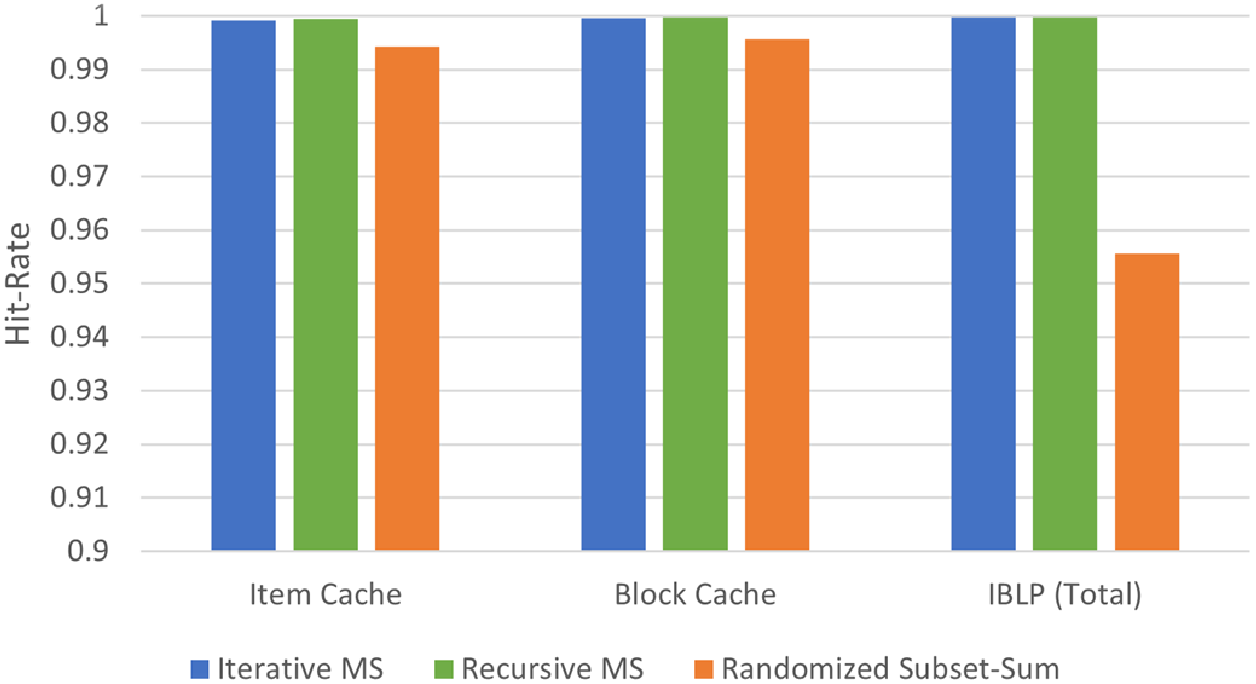
\includegraphics[height=2.8in]{figures/curtis_cache_hit_rates.png}
		\caption{Hit rates resulting from tests of the three cache configurations \cite{curtis}.}
	\end{figure}

	\vfill

	\begin{figure}[H]
		\centering
		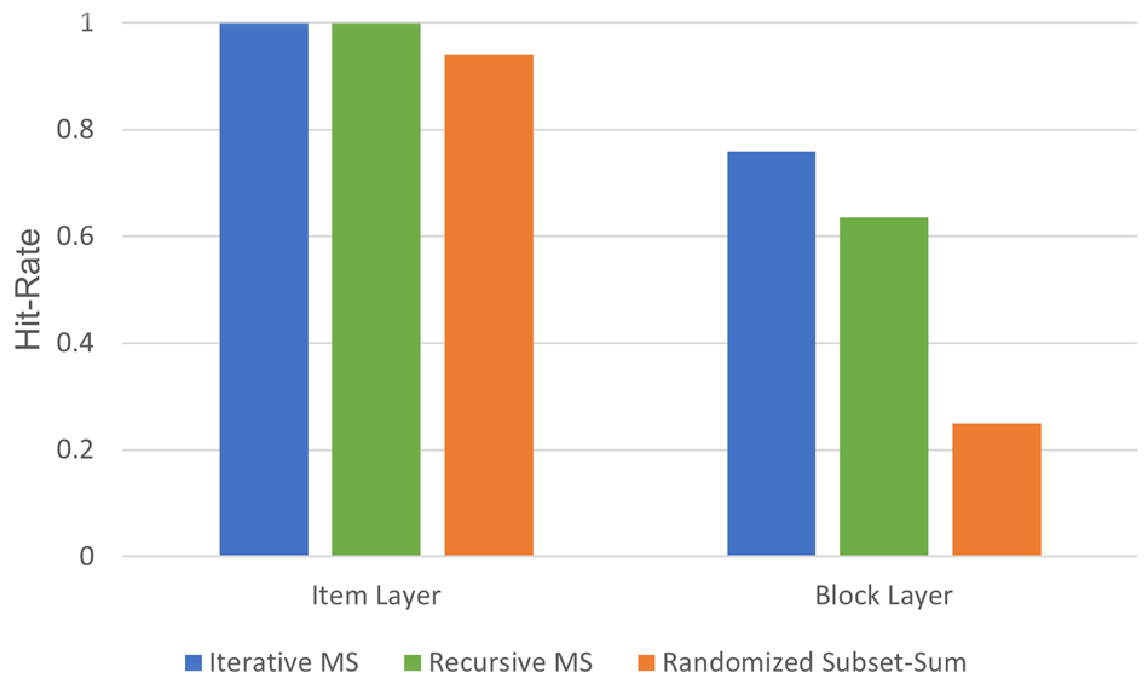
\includegraphics[height=2.8in]{figures/curtis_layer_hit_rates.png}
		\caption{Hit rates for the item and block layers of the IBLP cache \cite{curtis}.}
	\end{figure}

	\vfill

%%%%%%%%%%%%%%%%%%%%%%%%%%%%%%%%%%%%%%%%%%%%%%%%%%%%%%%%%%%%%%%%%
\chapter{Attempting a modular IBLP implementation}

\section{Overview of Gem5}

Gem5 is an open-source, community-led computer systems simulation project that describes itself as: \begin{quote}
	...a modular platform for computer-system architecture research, encompassing system-level architecture as well as processor microarchitecture \cite{gem5-about}.
\end{quote}

Gem5 began as two separate projects, m5 at the University of Michigan and GEMS at the University of Wisconsin, until the two simulators were merged in 2011 \cite{gem5-about}. It has an active development community and substantial documentation and resources, including a tutorial and extensive documentation on the Gem5 website, automatically-generated API documentation, and a full introductory course based on curriculum from CS 752 and CS 757 at the University of Wisconsin-Madison \cite{gem5-docs}.

I chose to use Gem5 to simulate a granularity-change cache due to the foundation and specific suggestions for future work provided by Curtis; in particular, the recommendation to use cache objects to examine the viability of IBLP \cite{curtis}.

	\subsection*{Caching subsystems}

	Due to its origins as a combination of m5 and GEMS, Gem5 contains two separate subsystems that can both be used to model caches. The primary difference between the two subsystems is their differing ability to model custom cache coherence protocols, the protocols used to keep multiple caches that store the same data consistent with each other in complex multiprocessor systems. Ruby also has extended functionality for modeling other more complex cache systems.
	
	Overall, the classic cache model from m5 provides simple, modular functionality for multi-level caches with an inflexible MOESI cache coherence protocol, whereas the Ruby cache model has more complex implementation details to allow implementation of customized cache coherence protocols. Specifically, classic caches are the much simpler model to implement because they only require object definitions in the Python config script \cite{gem5-tutorial}. On the other hand, Ruby caches require special files written in SLICC (Specification Language including Cache Coherence) to define coherence protocols \cite{gem5-ruby}. Furthermore, since Ruby's focus on cache coherence translates to a focus on multiprocessor systems running multithreaded programs, other components of a Ruby configuration are more complicated to include these additional features.

	Since the IBLP does not require specialized customization of cache coherence protocols and simulating IBLP with multithreading was not my focus, I opted to use the classic cache subsystem for my initial implementation.

	\subsection*{System configs}

	A configuration of a system in Gem5 is defined by a Python file in the ``configs'' directory, which imports various Gem5 components for the processor, clock, memory, busses, and all other parts of the system. The code in the config file establishes the relationships between these components and prompts the start of the simulation.

	Since a system to simulate is defined and run through such a config file, I will frequently refer to the primary Python implementation of a system as its config.

	To run a config, the path to this file is given to the appropriate build command for the config's architecture, along with any arguments such as the path of the script to simulate; for example, running \verb`build/X86/gem5.opt configs/my_config.py` simulates the system defined in \verb`my_config.py` using the compilation of Gem5 for an X86 system with \verb`.opt` indicating both optimizations and debug messages are enabled.

	\subsection*{Measuring statistics}

	Since Gem5 is intended for systems research, it provides a thorough report of statistics from a simulation written to \verb`gem5/m5out/stats.txt` at the termination of the simulation. This includes statistics for every object that is a member of the System object.

	For the purpose of analyzing a granularity-change cache simulation, \verb`stats.txt` provides hit and miss rate statistics for all caches in the system.

\section{Classic cache implementation}

	I began by implementing a nestled cache structure using classic Gem5 caches. This involved first building a simple cache configuration following the Gem5 documentation's ``Getting Started'' tutorial, then modifying the cache bus configuration to support a nestled block layer and writing a wrapper program to perform trials and collect data from the simulation (see Appendix A for code).

	\subsection*{System class}

	For the purpose of organizing and modularizing the facets of the Gem5 system configuration that are peripheral to the IBLP implementation, such as processor initialization and simulation execution, I implemented the system setup in a new class, \verb`StreamlinedSystem`. This class inherits the Gem5 \verb`System` class and adds the following methods to take care of setting up the components of a typical system for simulation and piecing together the components of the IBLP cache:

	\begin{itemize}
		\item \verb`__init__(self)` sets up the system attributes that are needed for setting up other features: clock, voltage, memory mode and ranges, cpu, and busses for between L1 and L2 caches.
	
		\item \verb`setup_caches(self, cache_type)` sets up and connects busses to the caches: the L1 instruction and data caches, which have constant configurations, and the L2 cache, which is configured as either an Item, Block, or IBLP cache.
	
		\item \verb`setup_memory(self)` sets up the main memory and connects it to the L2 cache bus.
	
		\item \verb`run(self, binary)` sets the simulation up to run as a process, and runs it.
	\end{itemize}

	The specific commands for of most of these steps, except for \verb`setup_caches`, are adapted from the Gem5 tutorial \cite{gem5-tutorial}.

	\subsection*{Cache objects}

	A basic classic cache configuration requires minor setup of cache objects and busses; this encompasses L1 data and instruction caches, which are specialized caches with ports specified in the System object, and a general L2 cache which I adapted into a nestled item and block cache:

	\begin{itemize}
		\item \verb`L1Cache`, \verb`DataCache`, and \verb`InstructionCache` are adapted from the Gem5 basic caches tutorial to mimic the typical on-processor data and instruction caches in an ordinary system.
	
		\item \verb`L2Cache` contains the attributes of a typical L2 cache that are shared by both item and block caches.
	
		\item \verb`ItemCache` and \verb`BlockCache` inherit from \verb`L2Cache` and set up the structure for the two-part IBLP cache.
	
		\item \verb`IBLPCache(ItemCache)` simulates an IBLP cache by using an item cache, connected on the memory-side to a block cache, with attributes set so that there is minimal latency between these two caches. The method \verb`connectMemSideBus` is altered to connect the block layer to the memory bus, to imitate the way the memory connects to layers in the IBLP cache model.
	\end{itemize}

	\subsection*{Variable parameters}

	Since there are a number of parameters of the cache objects that should be adjusted and fine-tuned during testing, I created \verb`options.json` to be read by the file where the cache objects are defined, and used to set cache attributes accordingly.

	\subsection*{Wrapper script}

	The wrapper file \verb`main.py` runs Gem5 with the config and collects the relevant statistics from \verb`stats.txt` at the end of each simulation.

	The wrapper takes the three arguments to customize trials: the path to the binary of the script to simulate, the cache models to be tested (out of Block, Item, and IBLP), and the number of trials to run of each cache type.

\section{System-scope granularity limitation}

	The crucial limitation of my initial classic cache implementation is that it relies on Gem5 having a way, such as through a cache object attribute, to specify the line size for any given layer of memory.

	Instead, Gem5 sets an attribute for line size at the level of the \verb`System` class, and all cache objects connected to the system inherit that value. This prevents any possibly implementation of granularity-change caches in classic caches without modification of Gem5's \verb`System` and \verb`Cache` classes to allow specification of a larger line size for memory.

	\subsection*{Packet access scope}

	One possible workaround to the system-wide line size would be to access memory packets directly in the block cache and convert their granularity, such as is done in the Curtis block cache. However, the python level of implementation used for configs does not support directly accessing packets; it only allows bus and port attributes of the system to be connected in the config, and all actual packet manipulation is done by C++ methods packaged behind Gem5's object libraries.

	\subsection*{Next steps}

	My original goal, stemming from the suggestion against further low-level modification of Gem5's source code, was to create an IBLP implementation using only Gem5's existing memory system customization features---thereby maintaining compatibility with the rest of Gem5's simulation options. So, in order to exhaust all paths to such an implementation, I opted to next explore the Ruby memory subsystem. Ruby's more involved implementation process and wider range of customization options suggested the possibility of granularity modification features or opportunities for workarounds not present in the classic cache subsystem.


\chapter{Exploring granularity workarounds in Gem5}

\section{The Ruby memory subsystem}

	Since my initial classic cache implementation failed to meet the requirements for simulating an IBLP cache, I turned to the Ruby cache system to see if its more detailed cache model included a way of overriding the system-wide line size requirement.

	\subsection*{Overview of Ruby}

	Ruby provides a detailed system for simulating a wide array of memory configurations, including ``inclusive/exclusive cache hierarchies with various replacement policies, coherence protocol implementations, interconnection networks, DMA and memory controllers'', and more \cite{gem5-ruby}.

	\begin{figure}[h]
		\centering
		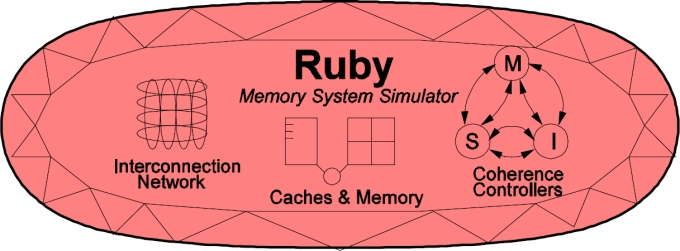
\includegraphics[width=4.5in]{figures/ruby.jpg}
		\caption{A graphic from GEMS visualizing Ruby's components \cite{gem5-ruby}.}
	\end{figure}

	Ruby's emphasis on highly configurable memory means it is mostly used specifically for research on cache coherence or otherwise complex interconnected memory systems. For my purpose, a simple but realistic memory system is sufficient to model IBLP, so most of the features of a Ruby cache system are unnecessary. However, implementation of a granularity-change-capable cache in Ruby would provide countless options for future research studying the intersection of granularity-change in caches with other complicating variables.

	\subsection*{Cache coherence specification}

	Ruby specifies cache coherence protocols using ``Specification Language for Implementing Cache Coherence'' (SLICC). These files are written in the ``src'' directory, and have to be compiled with a new build of Gem5, unlike configs. They do not provide any interaction with memory allocation that would allow for manipulation of cache granularity.

	\subsection*{Ruby architecture}

	Unlike classic caches, where cache objects are each individually connected with the system, Ruby cache objects are defined as cache controllers within a network and configured within a cache system.
	
	In the example from ``Learning Gem5'', the cache system named \verb`MyCacheSystem` is configured with a \verb`L1Cache` that inherits \verb`L1Cache_Controller`, a \verb`DirController` that inherits \verb`Directory_Controller`, and a memory network \verb`MyNetwork` inheriting \verb`SimpleNetwork` \cite{gem5-tutorial}.

	Since the matter of implementing granularity-change caching only concerns the architecture within a particular cache, only the \verb`L1Cache` is of significance. The \verb`L1Cache` object is defined with the following methods: \begin{itemize}
		\item \verb`versionCount` and \verb`getBlockSizeBits` are simple helpers for \verb`__init__`
		\item \verb`__init__` initializes the memory controller by defining its memory and connecting it to the system components
		\item \verb`sendEvicts` and \verb`connectQueues` manage components of cache coherence
	\end{itemize}

	Within \verb`__init__`, the memory definition provides the only config-level mention of block size: \begin{verbatim}
self.cacheMemory = RubyCache(
    size="16kB", assoc=8, start_index_bit=self.getBlockSizeBits(system)
)\end{verbatim}

	The helper \verb`getBlockSizeBits` here is a simple conversion of the system-level line size value, and thus can't be manipulated to modify the line size since it only determines the start bit offset. There is no evidence that Ruby offers any opportunities to manipulate individual-cache line size not present in a classic cache.

	\subsection*{Limitations}

	Since the Ruby caches, like the classic caches, operate under the assumption of a constant system-wide line size, there is no evident way to modify the granularity of individual memory layers using Ruby without extensive modification, to the degree of the Curtis block cache implementation or greater.

	Furthermore, the complexity of the Ruby subsystem is such that it would not be advisable to implement IBLP in Ruby unless specifically for the purpose of studying granularity-change caching in conjunction with features specific to Ruby, such as cache coherence.

\section{Granularity scope in the source code}

	The final possibility of implementing IBLP using existing Gem5 cache objects would be if relatively small modifications could be made to the Gem5 source code to change the granularity parameter, where it receives the system-assigned line size, to instead use a custom line size value.

	\subsection*{Cache interface source code}

	I began by inspecting the Python interface for the classic cache base object, defined in \verb`gem5/src/mem/cache/Cache.py`. This file contains Python interfaces for the following C++ classes:
	\begin{itemize}
		\item \verb`Clusivity`, an enum type object used to specify the behavior of a cache in regard to upstream caches as ``mostly inclusive'' or ``mostly exclusive''.
		\item \verb`WriteAllocator`, which is used for allocating memory for cache writes and invokes \verb`Parent.cache_line_size` to set its own \verb`block_size` attribute.
		\item \verb`BaseCache`, the parent class from which other cache objects inherit basic functionality.
		\item \verb`Cache`, the object used to create L1 and L2 caches in a config.
		\item \verb`NoncoherentCache`, to use as a last-level cache in multiprocessor systems.
	\end{itemize}

	At the interface level alone, the most that could be done to alter granularity of a specific cache is to overwrite \verb`WriteAllocator.block_size` with a new parameter, either passed down through the `Cache` constructor or through the system object as \verb`Parent` the same way that \verb`cache_line_size` is passed. This alteration would be required in conjunction with modification of all relevant C++ class definitions.

	\subsection*{Cache class definition source code}

	The C++ source code for the \verb`Cache` object, found in \verb`gem5/src/mem/cache/cache.cc`, contains definitions for 22 methods, many of which invoke inherited \verb`BaseCache` methods. These methods handle the actual passing of packets in and out of caches, including details of timing, eviction behavior, and snooping.

	The only reference to the system-level line size is where the \verb`Cache` constructor passes it to its parent `BaseCache`, on line 70 with:
	\begin{verbatim}
Cache::Cache(const CacheParams &p)
    : BaseCache(p, p.system->cacheLineSize()),
      doFastWrites(true)
	\end{verbatim}
	This parameter of \verb`BaseCache` is then used to set the attribute \verb`blkSize`. It would thus be simple to overwrite the value of \verb`blkSize` with a cache-specific custom granularity by replacing this use of \verb`p.system->cacheLineSize()` with either a custom system attribute or new constructor parameter.

	The use of block size following this appears well-contained to the scope of the \verb`Cache` class, only being used through the attribute \verb`blkSize`, which is referenced 15 times in \verb`cache.cc`. It is frequently used in conjunction with the \verb`Packet` method `getSize()`, and is only used in the context of packet operations.
	
	A cursory inspection of \verb`gem5/src/mem/cache/base.cc`, which contains the definitions for both \verb`BaseCache` and \verb`WriteAllocator`, shows similar usage and no references to the system-level line size via \verb`p.system->cacheLineSize()`. The base cache does have access to \verb`system` and its attributes, but only uses this in the context of handling requestors.
	
	From a cursory inspection of the \verb`Packet` source code in \verb`gem5/src/mem/packet.cc`, the \verb`Packet` class appears to be well-contained as well, with no evidence to suggest it would interfere with modification of higher-level objects.

	\subsection*{Compilation time}

	My initial attempts at modifying granularity definition in the Gem5 source code were limited somewhat by an unusually long compilation time. According to the Gem5 documentation, it is normal for compilation to take longer than 15 minutes \cite{gem5-build}. My system consistently took 20 minutes or more prior to even terminating with compilation errors, and longer for full compilation. Since system configurations such as the classic and ruby cache configs are implemented in Python and then run by the simulator, the simulator itself only needs to be compiled once, regardless of how often the configuration scripts are changed; so, the long build time is not typically an issue. However, since modifying and testing changes to the source code itself requires Gem5 to be recompiled each time modifications are made before those changes can be tested, a long build time makes the process of modifying Gem5's source code significantly more tedious---especially for such large changes that would require extensive debugging.

	\subsection*{Limitations}

	There are a few points of complication to attempting to modify Gem5's cache object source code, namely the implementation details of translating packet granularity, and the potential for errors caused by widespread access to system-level attributes.
	
	Since Gem5 is not built to accommodate translating memory packets between granularity, setting a different line size between cache layers will result in fatal errors unless packets are transformed between layers. This could potentially be solved with a custom cache bus, but only if the Gem5 source code is sufficiently modular that the modification of line size at the memory level would not interfere with line size at the processor level.
	
	Gem5 does have excellent modularity at the configuration level, as far as the ability to mix-and-match components, but modification of these components' source code in regard to system-level attributes is complicated by the fact that most low-level objects inherit access to system-level attributes. This makes it challenging to isolate objects from attributes of the \verb`System` instance, and makes it unlikely that the line size of an individual cache could be modified without identifying and accounting for all reference to the \verb`System` object's line size at lower levels.

	A cursory search using \verb`grep -r "p.system->cacheLineSize"` in \verb`gem5/src` shows only 11 references to \verb`p.system->cacheLineSize`, so replacing each of these instances could be doable. However, given the likelihood of unforeseen impacts on peripheral components, in practice this would likely be a much more daunting task to implement and troubleshoot.
	
	In conjunction with Gem5's relatively long compilation time, this suggests that even barring unforeseen complications, modifying the Gem5 source code to allow for variable granularity would be a substantially challenging and time-consuming task.

%%%%%%%%%%%%%%%%%%%%%%%%%%%%%%%%%%%%%%%%%%%%%%%%%%%%%%%%%%%%%%%%%
\chapter{Conclusion}

\section{Results of this research}

	Based on my research on implementing IBLP in Gem5, I conclude that a high-level implementation of a granularity-change cache is not possible in Gem5 due to the system-level definition of line size and closed interface at the configuration level.
	
	An initial look at the Gem5 source code suggests that modifying Gem5 to support multi-granularity caches may be possible. I provide cursory analysis of the challenges involved to explore the viability of this as an approach for future research in granularity-change cache simulation.

	\subsection*{The classic cache}

	The original idea of a nestled classic cache is supported in Gem5's classic cache subsystem at the structural level, as shown by my initial implementation attempt. However, due to the system-level definition of cache line size preventing assignment of differing granularities to individual caches, the nestled cache structure is unable to represent the core functionality of different-granularity layers necessary for a granularity-change cache.

	\subsection*{The Ruby cache}

	Despite the Ruby subsystem's expanded set of features for memory customization, I found that since Ruby depends on the same system object as the the classic cache, it suffers from the same fundamental limitation as the classic cache due to the system-wide line size requirement.

	\subsection*{Source code and system-scope granularity}

	My exploration of granularity definition in Gem5's source code revealed challenging interdependence of objects reliant on system-level attributes. On a cursory search, the system granularity attribute does not appear to have more references in the source code than could reasonably be located and individually modified. However, the likelihood of unanticipated impacts of these changes on other components in the system is high, and would likely require extensive troubleshooting. The relatively long build time of Gem5 adds some additional difficulty to this prospect.

	Aside from removing the system cache line size attribute, packet translation between granularities would need to be implemented; this was already done by the Curtis thesis for the block cache, and thus must be reasonably doable. Incorporating this granularity translation into Gem5's existing cache objects may, however, introduce additional complications due to the greater complexity of Gem5's native caches compared to the Curtis block cache.

\section{Future work}

	Despite the inefficacy of Gem5 for the purpose of simulating the granularity-change caching with its current configuration features, further study of the granularity-change caching problem through simulation is still a promising area for future research. Future work could involve either building on my exploration of Gem5's source code to modify Gem5 with support for multi-granularity caches, or surveying other cache simulators and choosing one to develop a new granularity-change cache implementation for.

	\subsection*{Continuing with Gem5}

	If one were to continue to pursue use of Gem5 for granularity-change caching research, my recommendation would be an approach between mine and that of Curtis, which would involve modification of the Gem5 source code to remove the cache line size from the system scope. Once support for custom cache granularity was implemented, a nestled cache similar to what I proposed in chapter 3 could be used to simulate a granularity-change cache.
	
	This approach would require in-depth analysis of the Gem5 codebase, a glimpse of which is given in section 3.5, as well as C++ implementation for conversion of packets between granularities as Curtis did for part of the block cache. Given the scope of these changes, this would likely be a major project that would require familiarity with compiling, debugging, and testing a large open-source project.

	Emphasis should be put on maintaining support for Gem5's more realistic processors so that the simulation could be used for rigorous, realistic testing of performance using granularity-change caching.

	\subsection*{Other simulation options for granularity-change caching}

	If one wanted to more generally further the study of granularity-change caching through simulation, my suggestion would be a survey of other memory system simulation tools in terms of their applicable features. The 2020 paper ``A Survey of Cache Simulators'' by Brais et. al. provides a starting point for this route by comparing 28 popular simulators, including Gem5 and Zsim. 4 of those simulators---Gem5, Sniper, ESESC, and MacSim---had last been updated within a year of Brais et. al. being published, suggesting that these options had good ongoing support as of 2020 \cite{brais}.

	
%%%%%%%%%%%%%%%%%%%%%%%%%%%%%%%%%%%%%%%%%%%%%%%%%%%%%%%%%%%%%%%%%
\appendix

\chapter{Source code}

\section{Classic config}

\subsection*{Caches}
\lstinputlisting{code/caches.py}
\vstep

\subsection*{Config}
\lstinputlisting{code/config.py}
\vstep

\subsection*{System}
\lstinputlisting{code/system.py}
\vstep

\subsection*{Wrapper}
\lstinputlisting{code/classic_wrapper.py}
\vstep

\section{Ruby config}

Files were not modified significantly from those provided at \url{https://github.com/gem5/gem5/tree/ee6f1377d7c54422137dfa47cd4d73407814867d/configs/learning_gem5/part3}.

\section{Gem5 object source code}

Full source code for the Gem5 project can be found at \url{https://github.com/gem5/gem5/}. The version referenced for this thesis is 23.1.0.0.

\nocite{*}
\addcontentsline{toc}{chapter}{References}
\printbibliography[title=References]

\end{document}
